\section{Grobentwurf}
\subsection {Globaler Kontrollfluss}

Im folgenden Abschnitt erläutern wir den Kontrollfluss der fertigen, initialisierten Anwendung im Einsatz. Eine Visualisierung des Kontrollflusses und der entsprechenden Aktivitäten findet sich in Abbildung \ref{fig:Kontroll}. Wir unterscheiden bei der Bedienung des Systems in zwei Sichten: Mitarbeitersicht und Kundensicht. Die Mitarbeitersicht ist synonym mit Administrator zu verstehen. Wir gehen in dieser Betrachtung davon aus, dass das System im Einsatz und vollständig konfiguriert sowie initialisiert wurde.

\subsubsection{Mitarbeitersicht}
Mitarbeiter oder Administratoren bewegen sich im Backend der Anwendung. Bevor das System durch einen Mitarbeiter der Filiale bedient werden kann, ist es erforderlich sich einzuloggen. Nach erfolgreichem Login können die Mitarbeiter die verfügbaren Aktivitäten in einer Menüstruktur frei wählen. Einzig für die Durchführung der Aktivität nach Kriterium \textbf{/F0170/} ist es notwendig, dass die Anwendung mit einem zentralen Server kommuniziert.

\subsubsection{Kundensicht}
Die Bedienung der Anwendung aus Kundensicht ist deutlich weniger frei als für Mitarbeiter. Um es auch Menschen mit wenig Technikerfahrung zu ermöglichen das System erfolgreich zu bedienen, ist die Anzahl der Wahlmöglichkeiten stark begrenzt.\\
\noindent Formulare werden zuerst in einer Menüstruktur gesucht und danach ausgewählt. Ist ein Formular ausgewählt worden, besteht die Möglichkeit direkt zu drucken, oder die eGK einzulesen um bestimmte Daten in das Formular eintragen zu lassen. Wurde ein Formular gedruckt, springt das System auf die Startseite zurück.\\
\noindent Das starten eines Videoanrufs mit einem Mitarbeiter nach Kriterium \textbf{/F0050/} soll zu jedem Zeitpunkt im Aktivitätsverlauf möglich sein. Ebenso ist es jederzeit möglich, den Prozess abzubrechen und zur Startseite zurückzukehren.

\newpage


\begin{figure}[htp]
    \flushleft
    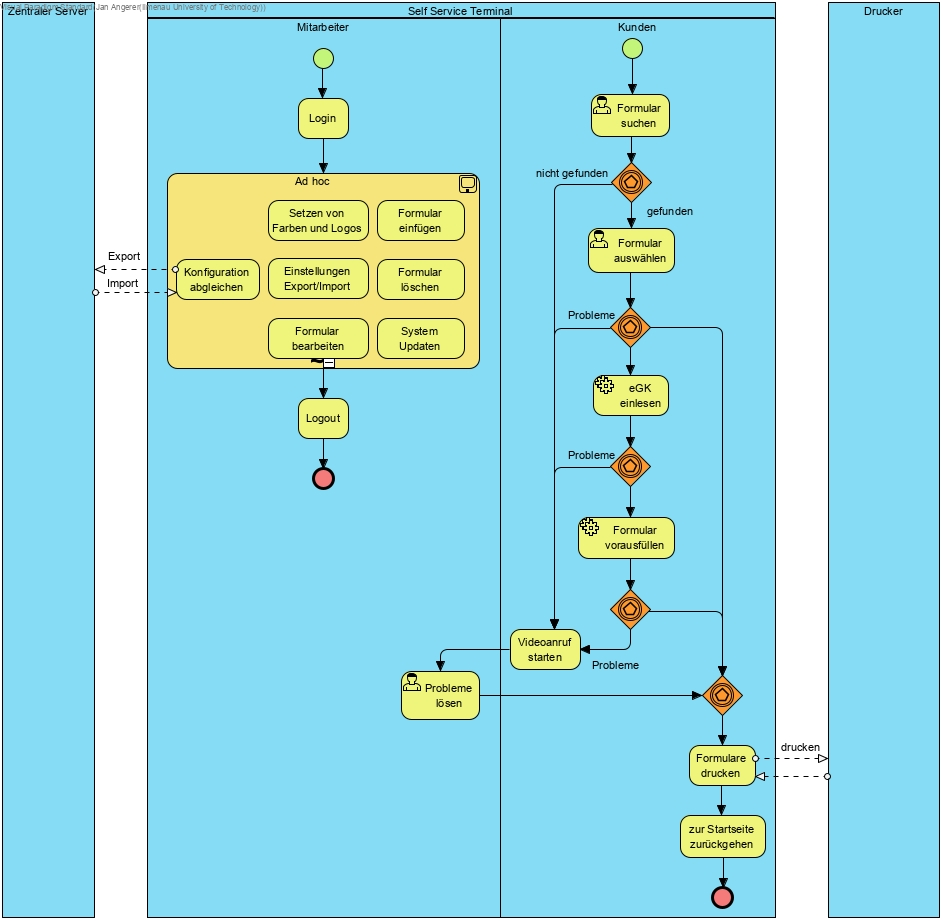
\includegraphics[width=14cm , height=13.5cm]{Kapitel/Bilder/SSTKontrollflussv2.jpg}
    \caption{Kontrollfluss der initialisierten Anwendung}
    \label{fig:Kontroll}
\end{figure}

\newpage
\subsection{Benutzeroberfläche}

\subsubsection{Dialogstruktur}

\textbf{Kundensicht:} \\

\noindent Für die erfolgreiche Bedienung des Systems ist es vor allem wichtig, dass die Kunden möglichst einfach die von ihnen benötigten Formulare finden. Eine Ordnerstruktur erscheint uns zu komplex, weswegen wir auf die Nutzung von Kategorien zurückgreifen. Die Dialogstruktur der Formularsuche ist in Abbildung \ref{fig:DiaglogKunden} beschrieben. Den Kunden werden immer nur die Optionen der horizontalen Ebene angezeigt, auf der sie sich aktuell befinden. Das Ziel ist möglichst wenige Schaltflächen gleichzeitig anzuzeigen. Die abgebildete Struktur orientiert sich an den zur Verfügung stehenden Formularen. Die Anordnung der Schaltflächen erfolgt dynamisch. Es ist also möglich weitere Formulare zu ergänzen. Die Formulierung \textit{Filter} in der Abbildung bezieht sich auf die Filterung der anzuzeigenden Formulare im Backend. \\

\noindent \textbf{Administratorsicht:} \\

\noindent Die konkrete Menüstruktur für die Administratoren sehen wir weniger kritisch als selbige Funktion für die Kunden. Es wird die Fähigkeit vorausgesetzt, sich in einer vordefinierten Menüstruktur zurechtzufinden. Entsprechend ist in Abbildung \ref{fig:DiaglogAdmin} unser Vorschlag für die Implementierung der Menüstruktur im Backend visualisiert. Nach erfolgreichem Login zeigt die Anwendung die Startseite an. Auf der Startseite kann gewählt werden, ob die Einstellungen der Anwendung selbst oder die Formulare gemanagt werden.

\newpage

\thispagestyle{empty}
\begin{landscape}
  \begin{figure}
      \centering
      \includegraphics[scale=0.5, center]{Kapitel/Bilder/Benutzeroberfläche_Kundev2.jpg}
      \caption{Dialogstruktur der Formularsuche aus Kundensicht}
      \label{fig:DiaglogKunden}
  \end{figure}
\end{landscape}

\newpage
\thispagestyle{empty}
\begin{landscape}
  \begin{figure}
      \centering
      \includegraphics[scale=0.6, center]{Kapitel/Bilder/BenutzeroberflächeAdminv2.jpg}
      \caption{Dialogstruktur aus Adminsitratorsicht}
      \label{fig:DiaglogAdmin}
  \end{figure}
\end{landscape}
\newpage

\subsubsection{Bildschirmlayout}

In Abbildung 6 ist ein Beispiel für das fertige Bildschirmlayout zu sehen. Es handelt sich um das Ergebnis eines Medienprojekts an der TU Ilmenau. Zusätzlich zu den gezeigten Schaltflächen, fügen wir einen Button ein, der direkt zurück zum Startbildschirm führt. Die Implementierung einer Schaltfläche zum Starten eines Videoanrufs ist optional.

\begin{figure}[htp]
    \centering
    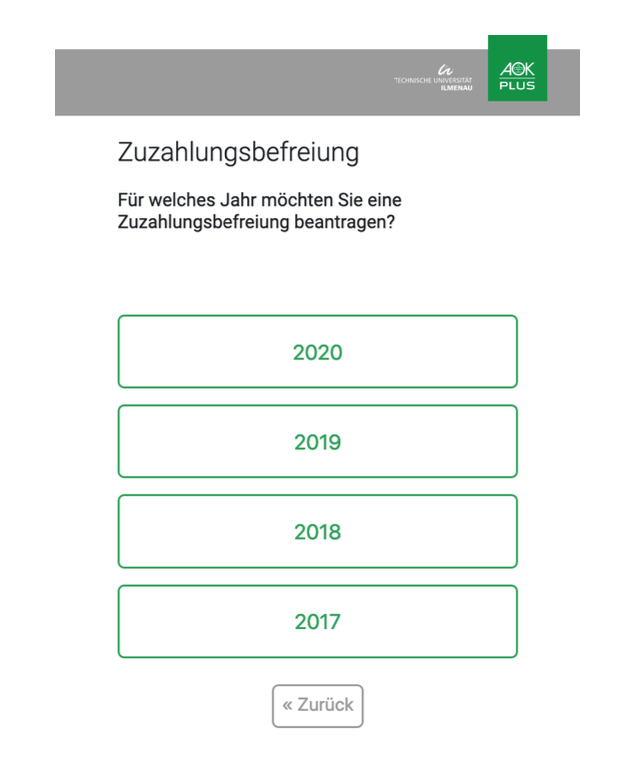
\includegraphics[width=10cm , height=12cm]{Kapitel/Bilder/Interface.png}
    \caption{Benedikt Bieberle, Niclas Deppisch und Robert Schwartz, "`Prototypische Entwicklung eines Self-Service-Terminals für Wartebereiche von Krankenkassenfilianen"', Medienprojekt TU Ilmenau, Mai 2020}
    \label{fig:Interface}
\end{figure}



\newpage



